\chapterimage{header.jpg}
\bigskip
\chapter{Building the SWAN}

 SWAN uses the \textit{SWAN.EDT} file to read the grid (\textit{swan\_coord.grd}) and bathymetry (\textit{swan\_bathy.bot}) files. 
It is also possible to define a numerical grid within the \textit{SWAN.EDT} and indicate the bathymetry file that will be read and associated 
with the defined grid.
\bigskip

 As an example, SWAN files will be created from the ROMS grid, but without the initial condition data.
\bigskip

 For SWAN boundary conditions, the wind fields will come from the WRF. Without the
the boundary files information, the simulated waves will be generated only within the boundary of the domain, disregarding the energy that
is leaving or entering the grid.
\bigskip

 We will use the MATLAB script, \textit{make\_swan.m}, to generate the files. The script is located at:
\bigskip

\begin{bashcode}
/home/name.surname/repositorio/SWAN_scripts
\end{bashcode}
\bigskip

 As shown in Figure \textcolor{bleu_cite}{\ref{makeswan}}, the script has the following construction:
\bigskip

\begin{figure}[H]
    \centering
    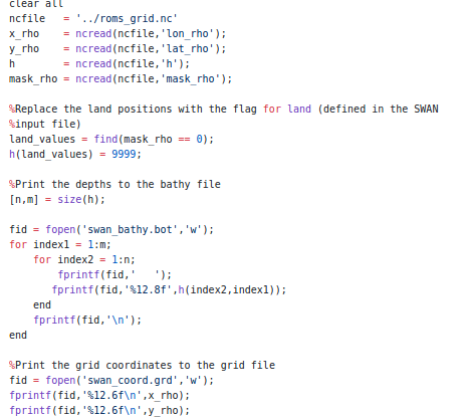
\includegraphics[width=0.47\textwidth]{makeswan.png}
    \caption{\textit{make\_swan.m} script.}
    \label{makeswan}
\end{figure}
\bigskip

 To generate the two SWAN files, search over in the script for the variable \textit{ncfile} and change the directory
to the path where your ROMS grid is.
\bigskip

 Run the script and the two files will be created: \textit{swan\_coord.grd} and \textit{swan\_bathy.bot}.
The two files must be placed inside your project folder.
\bigskip

\chapter{Building the Budgell's Sea Ice Model}
\bigskip

Since the sea ice model is fully coupled to ROMS, therefore, after generating the conditions of the
ROMS with ice data (see Section \textcolor{bleu_cite}{\ref{model2romssec}}), you can activate the sea ice model to be incialized too.
Just modify the ROMS \textit{.h} file in your project. According to \textcite{hedstrom2018}, you can
add the following options into the \textit{.h} file, as shown in Figure \textcolor{bleu_cite}{\ref{hiceroms}}:
\bigskip

\begin{itemize}
    \item \textbf{ICE\_MODEL}: defines the sea ice model;
    \item \textbf{ANA\_ICE}: defines initial analytical conditions for sea ice;
    \item \textbf{ICE\_THERMO}: defines the ice thermodynamics;
    \item \textbf{ICE\_MK}: defines the \textcite{Mellor1989} ice thermodynamics. Currently, is the only choice;
    \item \textbf{ICE\_MOMENTUM}: defines the momentum component of the ice;
    \item \textbf{ICE\_MOM\_BULK}: defines the alternate ice-water stress computation;
    \item \textbf{ICE\_EVP}: defines the elastic-viscous-plastic rheology from \textcite{Hunke1997} and \textcite{Hunke2001};
    \item \textbf{ICE\_QUAD\_STRENGTH}: defines the quadratic ice strength from \textcite{Overland1988};
    \item \textbf{ICE\_ADVECT}: defines the advection of ice tracers;
    \item \textbf{ICE\_SMOLAR}: defines the MPDATA use for ice tracers. Currently, it is the only option;
    \item \textbf{ICE\_UPWIND}: defines the upwind advection;
    \item \textbf{ICE\_BULK\_FLUXES}: define the ice part of bulk flux computation;
    \item \textbf{ICE\_DIAGS}: defines the diagnosis of sea ice;
    \item \textbf{ICE\_SHOREFAST} : defines the simple shorefast-ice algorithm from \textcite{Budgell2005};
    \item \textbf{ICE\_I\_O}: defines to allow light into the ice as heat;
    \item \textbf{ICE\_CONVSNOW}: defines the conversion of flooded snow to ice.
\end{itemize}
\bigskip

\begin{figure}[H]
    \centering
    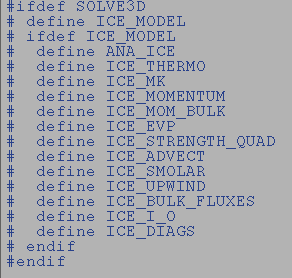
\includegraphics[width=0.3\textwidth]{hiceroms.png}
    \caption{Screenshot of ROMS \textit{.h} file}
    \label{hiceroms}
\end{figure}
\bigskip

\begin{tcolorbox}[enhanced,
    grow to left by   = 0cm,
    grow to right by  = 0cm,
    enlarge top by    = 0cm,
    enlarge bottom by = 0cm,
    tcbox raise base,
    boxrule           = 1.0pt,
    left              = 18mm,
    colframe          = green!50!black,coltext=green!25!black,colback=green!10!white,
    overlay           = {\begin{tcbclipinterior}\fill[green!75!blue!50!white] (frame.south west)
      rectangle node[text=white,font=\sffamily\bfseries\footnotesize,rotate=0] {WARNING} ([xshift=18mm]frame.north west);\end{tcbclipinterior}}]
For more information about the sea-ice model, it is recommended to read \textcite{hedstrom2018}.
\end{tcolorbox}
\bigskip

 Get the \textit{.in} file for the sea ice model. Copy the file \textit{ice.in} into the Kerana repository and add it to your project.
\bigskip

\begin{bashcode}
    /home/name.surname/repositorio/ICE_scripts
\end{bashcode}
\bigskip
    
 Modify the ROMS \textit{.in} file, pointing to the \textit{ice.in} into the variable \textit{IPARNAM}:
\bigskip

\begin{bashcode}
nedit ocean.in
IPARNAM =  ice.in
\end{bashcode}